%subsection{\acrshort{mpi}-\acrshort{openmp} Tuning of \acrshort{mumps} Library}
\subsection{Hybrid \acrshort{mpi}/\acrshort{openmp} Computing}

\label{subseq:mpi-openmp}


As it was mentioned in Section \ref{subseq:mumps-review}, the development of \acrshort{mumps} began in 1996 when message-passing programming paradigm dominated in parallel computing. Therefore, the library originally was designed only for distributed-memory machines.\\

In 2010,  \citeauthor{chowdhury2010some} published their first experiments and some issues, in \cite{chowdhury2010some}, of exploiting shared memory parallelism in \acrshort{mumps}. The authors showed that it was possible to achieve some improvements in multicore systems using multi-threading, given a purely \acrshort{mpi} application. However, later \citeauthor{l2013introduction} mentioned, in \cite{l2013introduction}, that adaptation of the existing code for \acrshort{numa} architecture was still a challenge because of memory allocation, memory affinity, thread pinning and other related issues.\\


In spite of an advantage of natural data locality of message-passing applications, a general motivation for switching to a hybrid mode, a mixed \acrshort{mpi}/\acrshort{openmp} process/thread distribution, is to reduce communication overheads between \acrshort{mpi} processes. According to the profiling results obtained by \citeauthor{chowdhury2010some}, \acrshort{mumps} contained four main regions of shared-memory parallelization, namely: 

\begin{enumerate}

	\item \acrshort{blas} Level 1, 2, 3 operations during both factorization and solution phases \label{openmp-blocks-1}
	
	\item Assembly operations, where contribution blocks of children nodes are assembled at the parent level \label{openmp-blocks-2}
	
	\item Copying contribution blocks during stacking operations \label{openmp-blocks-3}
	
	\item Pivot search operations \label{openmp-blocks-4}

\end{enumerate}


Almost all customized \acrshort{blas} libraries, for example Intel MKL and OpenBLAS, are multi-threaded and can efficiently work in shared-memory environment. Hence, parallelization of region \ref{openmp-blocks-1} can be achieved by linking a suitable \acrshort{blas} library whereas regions \ref{openmp-blocks-2}, \ref{openmp-blocks-3} and \ref{openmp-blocks-4} can be multi-threaded by inserting appropriate \acrshort{openmp} directives above the corresponding loop statements.\\


A detailed review of works \cite{l2013introduction} and \cite{chowdhury2010some} reveals that, in general, a pure \acrshort{openmp} or mixed \acrshort{mpi}/\acrshort{openmp} strategy can reduce run-time of \acrshort{mumps}. On average, factorization time is reduced by \textbf{14.3\%} and in some special cases improvements reach about \textbf{50.4\%}, according to analysis performed on data provided in the papers. However, at the same time, the results also show that sometimes a flat-\acrshort{mpi} mode can significantly outperform other hybrid mixed strategies.\\


By and large, the results show two important aspects. Firstly, performance of a specific strategy depends heavily on a resulting assembly tree and thus on a matrix sparsity pattern and applied fill reducing reordering. Secondly, it is not possible to guess in advance which strategy gives the best parallel performance without detailed information about the tree structure and computational cost per node. \citeauthor{l2013introduction} showed that performance of a particular mode dependeds on a ratio of large and small fronts. For example, they noticed that more threads per \acrshort{mpi} process resulted in better parallel performance in case of high ratios. On the other hand, they observed the absolutely opposite result with relatively small ratios. Unfortunately, \citeauthor{l2013introduction} did not provide any quantitative measure for the notion of small and large ratios in  \cite{l2013introduction}.\\ 


It is also interesting to notice that parallelization of region 1 using a multi-threaded \acrshort{blas} library gives the most of the parallel performance improvement for mixed or pure \acrshort{openmp} strategies, according to analysis of results from \cite{l2013introduction}. Whereas,
multi-threading of regions 2, 3, 4 has only a small positive effect i.e it reduces numerical factorization run-time by only \textbf{0.66\%} on an average.\\



This outcome is expected because \acrshort{blas} subroutines, especially level 3, re-use data stored in caches as much as possible and thus achieve high ratios of floating point operations per memory access which is essential for efficient multi-threading. Meanwhile, regions 2, 3, 4 mainly perform initialization of variables, data movements and executions of \textit{if-statements} which always result in low computational intensity.\\

%\todo{consider that paragraph}
%Additionally, it is worth noticing that both works, \cite{chowdhury2010some} and \cite{l2013introduction}, were mainly focused on the numerical factorization phase assuming that both analysis and solution phases do not take lots of computational time. In spite of credibility of this assumption, it still should be pointed out the solution phase runs faster in case of flat-\acrshort{mpi} mode. This fact becomes even more interesting because, in our case, a system with multiple right-hand sides has to be solved in order to generate a preconditioner.\\


We have to admit that both works, \cite{chowdhury2010some} and \cite{l2013introduction}, are relatively old and the analysis above may be not complete and full. Because \acrshort{mumps} is a dynamic developing project, we can expect that adaptation of shared-memory parallelization in \acrshort{mumps} has been significantly advanced since that time. Since the 4th release of \acrshort{mumps} library, the developers have persistently recommended to use only hybrid strategies e.g. \textit{one \acrshort{mpi} process per socket and as many threads as the number of cores}, \cite{mumps-manual}.\\


As an initial test, we compared an influence of both Intel MKL and OpenBLAS libraries on parallel performance of \acrshort{mumps} using \acrshort{grs} matrix set only. In order to pin \acrshort{openmp} threads in a correct way, without any conflicts between them, the following \acrshort{openmp} environment variables were set as follows:

\begin{itemize}
	\item OMP\_PLACES=cores
	\item OMP\_PROC\_BIND=spread
\end{itemize} 


During the testing, we found that sometimes execution time of \acrshort{mumps}-OpenBLAS configuration abnormality increased. For instance, in case of parallel factorization of matrix \textit{cube-645}, the increase reached almost \textbf{450\%} in contrast to the pure sequential execution. \\

\figpointer{\ref{fig:mumps-openblas-anomalies}}
\begin{figure}[htpb]
\centering
	\begin{tabular}{cc}
		\subfloat[k3-18]{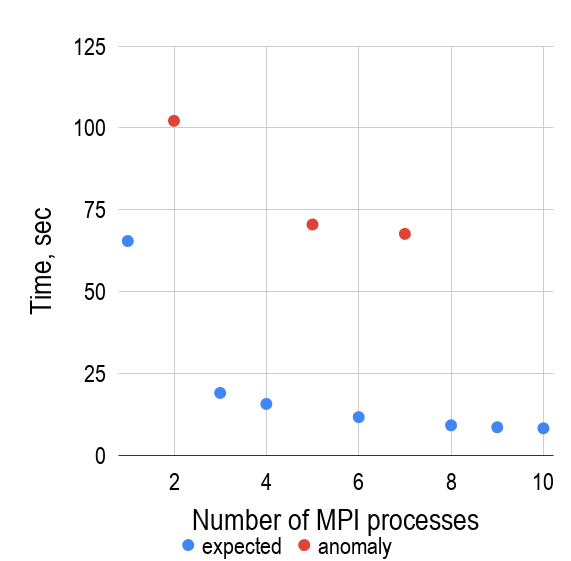
\includegraphics[width=0.4\textwidth]{figures/chapter-2/openmp-mpi/anomalies-k3-18.png}} &
		\subfloat[cube-645]{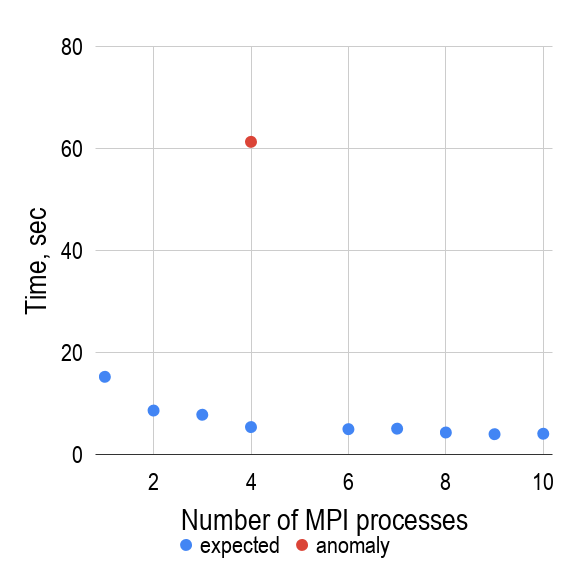
\includegraphics[width=0.4\textwidth]{figures/chapter-2/openmp-mpi/anomalies-cube-645.png}} \\
	\end{tabular}
	\caption[Anomalies of parallel executions of \acrshort{mumps}-OpenBLAS configuration during factorizations of large-sized \acrshort{grs} matrices]{Anomalies of parallel executions of \acrshort{mumps}-OpenBLAS configuration during factorizations of large-sized \acrshort{grs} matrices running with 2 \acrshort{openmp} threads per \acrshort{mpi} process}
	\label{fig:mumps-openblas-anomalies}
\end{figure}


Multiple conflicts between application and system threads were observed using \textit{htop} software as an interactive process viewer. Figure \ref{fig:mumps:openblas-thread-conflcit} shows a snapshot taken during factorization of matrix \textit{k3-18} running with 1 \acrshort{mpi} process and 20 threads.\\


\figpointer{\ref{fig:mumps:openblas-thread-conflcit}}
\begin{figure}[htpb]
  \centering
  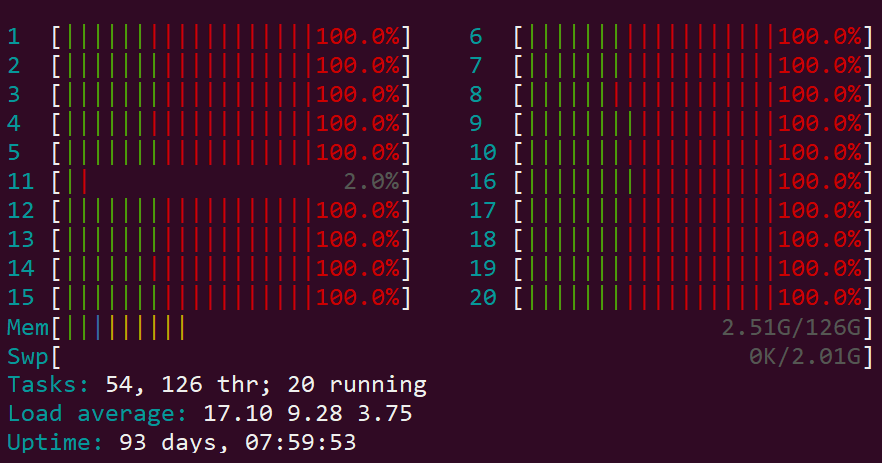
\includegraphics[width=0.75\textwidth]{figures/chapter-2/openmp-mpi/thread-conflict.png}
\caption[Thread conflicts of \acrshort{mumps}-OpenBLAS configuration detected during parallel factorization of  matrix \textit{k3-18}]{Thread conflicts of \acrshort{mumps}-OpenBLAS configuration detected during parallel factorization of matrix \textit{k3-18}, where green - application threads, red - system threads}
\label{fig:mumps:openblas-thread-conflcit}
\end{figure}


It is difficult to state what exactly caused such behavior. However, \citeauthor{chowdhury2010some} also reported about the same problem using GotoBLAS (OpenBLAS). They assumed that GotoBLAS created and kept some threads active even after the main threads returned to the calling application which could lead to interference with threads created in other \acrshort{openmp} regions \cite{chowdhury2010some}. For this reason, we decided to use only Intel MKL library for the rest of the study because there were no such thread-conflicts detected during operation of \acrshort{mumps}-Intel MKL configuration.\\


Only common mixed \acrshort{mpi}/\acrshort{openmp} strategies were tested in order to check an influence of shared-memory parallelism on parallel performance of \acrshort{mumps} as well as to limit an amount of testing. The following strategies were chosen: 20 \acrshort{mpi} - 1 thread (flat-\acrshort{mpi}), 10 \acrshort{mpi} - 2 threads, 4 \acrshort{mpi} - 5 threads, 2 \acrshort{mpi} - 10 threads, 1 \acrshort{mpi} - 20 threads (flat-\acrshort{openmp}). The tests were conducted on both \gls{hw1} and \gls{hw2} machines with the aim of checking whether  results would be consistent between different hardware running under different operating and environment settings. Results of testing are represented in Tables \ref{fig:mpi-omp-grs-hw1} \ref{fig:mpi-omp-grs-hw2}, \ref{fig:mpi-omp-suitesparse-hw1} and \ref{fig:mpi-omp-suitesparse-hw2} where numerical values are given in seconds.\\


%%%%%%%%%%%%%%%%%%%%%%%%%%%%%%%%%%%%%%%%%%%%%%%%%%%%
\begin{table}[h!]
\centering
\begin{tabular}{|c|c|c|c|c|c|c|}
\hline
\begin{tabular}[c]{@{}c@{}}Matrix\\ Name\end{tabular} & \begin{tabular}[c]{@{}c@{}}20 MPI\\ 1 thread\end{tabular} & \begin{tabular}[c]{@{}c@{}}10 MPI\\ 2 threads\end{tabular} & \begin{tabular}[c]{@{}c@{}}4 MPI\\ 5 threads\end{tabular} & \begin{tabular}[c]{@{}c@{}}2 MPI\\ 10 threads\end{tabular} & \begin{tabular}[c]{@{}c@{}}1 MPI\\ 20 threads\end{tabular} & \begin{tabular}[c]{@{}c@{}}Gain\\ w.r.t.\\ flat-MPI\end{tabular} \\ \hline
k3-18                                                 & \textbf{12.520}                                           & 12.630                                                     & 14.010                                                    & 18.020                                                     & 19.170                                                     & -                                                                \\ \hline
k3-2                                                  & 1.341                                                     & \textbf{1.250}                                             & 1.470                                                     & 1.671                                                      & 2.052                                                      & 1.073                                                            \\ \hline
cube-645                                              & \textbf{6.585}                                            & 6.859                                                      & 8.552                                                     & 12.010                                                     & 14.080                                                     & -                                                                \\ \hline
cube-64                                               & 0.756                                                     & \textbf{0.749}                                             & 0.874                                                     & 1.178                                                      & 1.354                                                      & 1.010                                                            \\ \hline
cube-5                                                & 0.181                                                     & 0.132                                                      & \textbf{0.104}                                            & 0.126                                                      & 0.117                                                      & 1.744                                                            \\ \hline
pwr-3d                                                & 0.130                                                     & 0.114                                                      & 0.0972                                                    & \textbf{0.077}                                             & 0.109                                                      & 1.691                                                            \\ \hline
\end{tabular}
\caption{Compassions of different hybrid \acrshort{mpi}/\acrshort{openmp} modes used for parallel factorization of \acrshort{grs} matrix set on \gls{hw1}}
\label{fig:mpi-omp-grs-hw1}
\end{table}



\begin{table}[h!]
\centering
\begin{tabular}{|c|c|c|c|c|c|c|}
\hline
\begin{tabular}[c]{@{}c@{}}Matrix\\ Name\end{tabular} & \begin{tabular}[c]{@{}c@{}}20 MPI\\ 1 thread\end{tabular} & \begin{tabular}[c]{@{}c@{}}10 MPI\\ 2 threads\end{tabular} & \begin{tabular}[c]{@{}c@{}}4 MPI\\ 5 threads\end{tabular} & \begin{tabular}[c]{@{}c@{}}2 MPI\\ 10 threads\end{tabular} & \begin{tabular}[c]{@{}c@{}}1 MPI\\ 20 threads\end{tabular} & \begin{tabular}[c]{@{}c@{}}Gain\\ w.r.t.\\ flat-MPI\end{tabular} \\ \hline
k3-18                                                 & 8.558                                                     & \textbf{7.819}                                             & 8.165                                                     & 11.330                                                     & 14.320                                                     & 1.095                                                            \\ \hline
k3-2                                                  & 1.168                                                     & \textbf{0.788}                                             & 0.956                                                     & 1.131                                                      & 1.651                                                      & 1.482                                                            \\ \hline
cube-645                                              & 5.735                                                     & \textbf{4.859}                                             & 6.069                                                     & 9.360                                                      & 11.040                                                     & 1.180                                                            \\ \hline
cube-64                                               & 0.805                                                     & \textbf{0.541}                                             & 0.664                                                     & 0.947                                                      & 0.918                                                      & 1.490                                                            \\ \hline
cube-5                                                & 0.241                                                     & 0.121                                                      & \textbf{0.093}                                            & 0.129                                                      & 0.126                                                      & 2.582                                                            \\ \hline
pwr-3d                                                & 0.234                                                     & 0.095                                                      & 0.098                                                     & \textbf{0.070}                                             & 0.094                                                      & 3.341                                                            \\ \hline
\end{tabular}
\caption{Compassions of different hybrid \acrshort{mpi}/\acrshort{openmp} modes used for parallel factorization of \acrshort{grs} matrix set on \gls{hw2}}
\label{fig:mpi-omp-grs-hw2}
\end{table}


%%%%%%%%%%%%%%%%%%%%%%%%%%%%%%%%%%%%%%%%%%%%%%%%%%%%
\begin{table}[h!]
\centering
\begin{tabular}{|c|c|c|c|c|c|c|}
\hline
\begin{tabular}[c]{@{}c@{}}Matrix\\ Name\end{tabular} & \begin{tabular}[c]{@{}c@{}}20 MPI\\ 1 thread\end{tabular} & \begin{tabular}[c]{@{}c@{}}10 MPI\\ 2 threads\end{tabular} & \begin{tabular}[c]{@{}c@{}}4 MPI\\ 5 threads\end{tabular} & \begin{tabular}[c]{@{}c@{}}2 MPI\\ 10 threads\end{tabular} & \begin{tabular}[c]{@{}c@{}}1 MPI\\ 20 threads\end{tabular} & \begin{tabular}[c]{@{}c@{}}Gain\\ w.r.t.\\ flat-MPI\end{tabular} \\ \hline
cant                                                  & 1.400                                                     & \textbf{0.990}                                             & 1.050                                                     & 1.605                                                      & 2.019                                                      & 1.414                                                            \\ \hline
consph                                                & 3.495                                                     & \textbf{2.652}                                             & 3.015                                                     & 3.706                                                      & 3.714                                                      & 1.318                                                            \\ \hline
memchip                                               & \textbf{7.470}                                            & 9.080                                                      & 13.301                                                    & 20.198                                                     & 45.800                                                     & -                                                                \\ \hline
PFlow\_742                                            & 26.802                                                    & 24.204                                                     & \textbf{21.897}                                           & 30.389                                                     & 54.501                                                     & 1.224                                                            \\ \hline
pkustk10                                              & \textbf{0.748}                                            & 0.879                                                      & 0.972                                                     & 1.459                                                      & 1.280                                                      & -                                                                \\ \hline
torso3                                                & \textbf{3.922}                                            & 4.285                                                      & 4.642                                                     & 5.603                                                      & 8.144                                                      & -                                                                \\ \hline
x104                                                  & \textbf{1.597}                                            & 1.644                                                      & 2.024                                                     & 3.208                                                      & 2.167                                                      & -                                                                \\ \hline
CurlCurl\_3                                           & 49.250                                                    & 44.120                                                     & \textbf{39.909}                                           & 43.311                                                     & 63.001                                                     & 1.234                                                            \\ \hline
Geo\_1438                                             & 478.101                                                   & 234.697                                                    & \textbf{151.603}                                          & 157.697                                                    & 158.102                                                    & 3.154                                                            \\ \hline
\end{tabular}
\caption{Compassions of different hybrid \acrshort{mpi}/\acrshort{openmp} modes used for parallel factorization of SuiteSparse matrix set on \gls{hw1}}
\label{fig:mpi-omp-suitesparse-hw1}
\end{table}




\begin{table}[h!]
\centering
\begin{tabular}{|c|c|c|c|c|c|c|}
\hline
\begin{tabular}[c]{@{}c@{}}Matrix\\ Name\end{tabular} & \begin{tabular}[c]{@{}c@{}}20 MPI\\ 1 thread\end{tabular} & \begin{tabular}[c]{@{}c@{}}10 MPI\\ 2 threads\end{tabular} & \begin{tabular}[c]{@{}c@{}}4 MPI\\ 5 threads\end{tabular} & \begin{tabular}[c]{@{}c@{}}2 MPI\\ 10 threads\end{tabular} & \begin{tabular}[c]{@{}c@{}}1 MPI\\ 20 threads\end{tabular} & \begin{tabular}[c]{@{}c@{}}Gain\\ w.r.t\\ flat-MPI\end{tabular} \\ \hline
cant                                                  & 2.128                                                     & \textbf{0.955}                                             & 1.011                                                     & 1.577                                                      & 2.058                                                      & 2.229                                                           \\ \hline
consph                                                & 3.840                                                     & \textbf{2.852}                                             & 3.111                                                     & 3.695                                                      & 3.897                                                      & 1.346                                                           \\ \hline
memchip                                               & \textbf{7.811}                                            & 7.816                                                      & 9.811                                                     & 15.160                                                     & 31.969                                                     & -
\\ \hline
PFlow\_742                                            & 24.190                                                    & 29.241                                                     & \textbf{19.686}                                           & 27.530                                                     & 55.431                                                     & 1.230                                                           \\ \hline
pkustk10                                              & 1.373                                                     & \textbf{0.904}                                             & 1.022                                                     & 1.421                                                      & 1.403                                                      & 1.520                                                           \\ \hline
torso3                                                & 4.733                                                     & \textbf{4.080}                                             & 4.483                                                     & 5.648                                                      & 8.217                                                      & 1.160                                                           \\ \hline
x104                                                  & 2.676                                                     & \textbf{1.597}                                             & 2.025                                                     & 3.204                                                      & 2.133                                                      & 1.676                                                           \\ \hline
CurlCurl\_3                                           & 39.890                                                    & \textbf{34.579}                                            & 38.620                                                    & 41.171                                                     & 67.760                                                     & 1.154                                                           \\ \hline
Geo\_1438                                             & ROM                                                       & ROM                                                        & ROM                                                       & ROM                                                        & ROM                                                        & ROM                                                             \\ \hline
\end{tabular}
\caption[Compassions of different hybrid \acrshort{mpi}/\acrshort{openmp} modes used for parallel factorization of SuiteSparse matrix set on \gls{hw2}\\]{Compassions of different hybrid \acrshort{mpi}/\acrshort{openmp} modes used for parallel factorization of SuiteSparse matrix set on \gls{hw2}, where ROM stands for Run Out of Memory}
\label{fig:mpi-omp-suitesparse-hw2}
\end{table}


%According to the results, we have noticed the optimal hybrid \acrshort{mpi}/\acrshort{openmp} mode locates near the saturation point of the corresponding flat-\acrshort{mpi} test. Therefore, search of an optimal mode can take considerable amount of time. It is needless to say that the mode varies from matrix to matrix and there is no way to predict the mode in advance. Moreover, the results show that performance gain is around \textbf{2.1\%} in case of \acrshort{grs} matrix set on \gls{hw1} hardware, excluding small test cases such as \textit{cube-5} and \textit{pwr-3d} where runs with 20 \acrshort{mpi} processes were slower in contrast to sequential execution. Much optimistic results were obtained for experiments conducted on \gls{hw2} machine were performance gain reached almost \textbf{31\%} for the same test cases.\\


%According to the results, we have noticed that an optimal hybrid \acrshort{mpi}/\acrshort{openmp} mode locates near the saturation point of the corresponding flat-\acrshort{mpi} test. Generally speaking, a location of the saturation point is specific for each matrix and, therefore, there is no way to predict a mode in advance. However, having known the point, an amount of testing can be considerably reduced by searching around and applying different mixed \acrshort{mpi}/\acrshort{openmp} strategies.\\

According to analysis of obtained results and flat-\acrshort{mpi} performance graphs from Subsection \ref{subseq:blas-comparison}, we have noticed that an optimal hybrid \acrshort{mpi}/\acrshort{openmp} mode locates near the saturation point of the corresponding flat-\acrshort{mpi} test. Generally speaking, a location of the saturation point is specific for each matrix and, therefore, there is no way to predict a mode in advance. However, having known the point, an amount of testing can be considerably reduced by searching around and applying different mixed \acrshort{mpi}/\acrshort{openmp} strategies.\\



The results show that average performance gain is around \textbf{2.1\%} in case of \acrshort{grs} matrix set for \gls{hw1} hardware, excluding small test-cases such as \textit{cube-5} and \textit{pwr-3d} from statistics. We consider these two scenarios, \textit{cube-5} and \textit{pwr-3d}, as specific ones because their execution time with 20 \acrshort{mpi} processes using flat-\acrshort{mpi} mode is originally slower in contrast to the sequential execution and, therefore, it is relevant to assume that the improvement came only from reducing of the \acrshort{mpi} process count. At the same time, much optimistic results were obtained from experiments conducted on \gls{hw2} machine where performance gain reached almost \textbf{31\%} for the same test-cases.\\



Results obtained with SuiteSparse matrix set demonstrate much better performance improvements from hybrid parallel computing obtained on both hardware. On average, execution time improves by more than \textbf{15\%} running tests on \gls{hw1} and approximately by \textbf{41\%} on \gls{hw2}, excluding \textit{Geo\_1438} from the statistics. The best result was obtained exactly in case of \textit{Geo\_1438} test-case on both machines where execution time dropped about \textbf{3 times} for all hybrid modes in contrast to the corresponding flat-\acrshort{mpi} one. We assume it may occur because of a high ratio of large and small fronts of this particular test-case.\\


According to the outcomes of testing, we have observed a negligible improvement in \acrshort{mumps} parallel performance from the application of the multi-threaded Intel MKL \acrshort{blas} library to \acrshort{grs} matrix set. Such unimpressive results can be explained with the same reasoning given in Subsection \ref{subseq:blas-comparison} i.e. lack of type 2 nodes. Moreover, in case of \acrshort{grs} matrix set, parallel efficiency drops significantly probably due to inefficient utilization of additional processing elements i.e cores. However, at the same time, results obtained using SuiteSparse matrix set have shown an advantage of hybrid parallel computing, especially in case of \textit{Geo\_1438} matrix factorization.\\


These contradictory results obtained from two different matrix sets second our reasoning about specifics of linear systems generated by \acrshort{athlet} software. Again, we presume that assembly trees resulted from \acrshort{grs} matrices are mostly formed with subtrees filled with type 1 nodes where each subtree is processed by a single \acrshort{mpi} process. Hence, parallel factorization of \acrshort{grs} matrices mainly gets benefit from \acrshort{mpi} parallelization that can be clearly observed from the results.\\



In this Subsection, we have discussed how \acrshort{mumps} adopts hybrid parallel computing. As it is in case of fill reducing reordering algorithm selection, Subsection \ref{subseq:fill-in-reordering}, it is not possible to find an optimal mixed \acrshort{mpi}/\acrshort{openmp} strategy in advance without performance testing. We have come to the conclusion that flat-\acrshort{mpi} mode is the best one for \acrshort{grs} matrix set and provided our reasoning for that. Generally speaking, there are 3 reasons to use this mode in our case. Firstly, the mode always resulted in more efficient hardware utilization. Secondly,  \acrshort{mumps}-Intel MKL configuration running with optimal hybrid \acrshort{mpi}/\acrshort{openmp} strategies can deteriorate performance gain obtained with \acrshort{mumps}-OpenBLAS flat-\acrshort{mpi} configuration, shown in Subsection \ref{subseq:blas-comparison}. Finally, efficient utilization of flat-\acrshort{mpi} strategy only demands to find an optimal \acrshort{mpi} process count i.e the saturation point on a performance graph. Hence, it leads to a significant reduction of testing due to a reduced number of parameters which are needed to be taken into account.\\
